\chapter{Proposed Methodology}
\label{Methodology}
\overridetextsize

\section{Noise-Aided Adversarial Example Detection (NAED) Method}
As observed during the experiments conducted in section \ref{sub:consistency}
and section \ref{sub:logits_differences}, the usage of Gaussian noise to alter
the efficacy of the perturbations present in adversarial examples is effective.
To build upon these observations, I propose a methodology to detect adversarial
examples that I describe in the remainder of this section.

This methodology, represented in figure \ref{fig:framework}, aims to compute two
scores, described in the following subsection, using the difference in
predictions before and after applying random noise to the input image space.
From the two scores computed for each input, we can determine if an input is
adversarial or not.

\begin{figure}[htp]
    \centering
    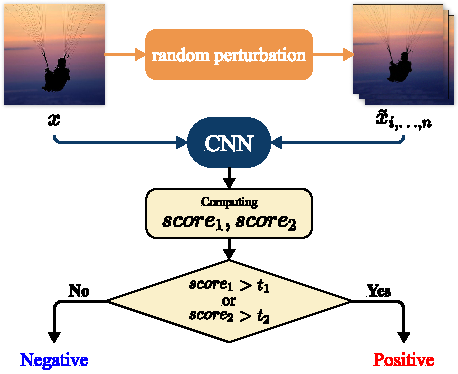
\includegraphics[clip,width=0.9\columnwidth]{Figures/methodology/Framework.pdf}%

    \caption{The framework of the discussed method.}
    \label{fig:framework}
\end{figure}

\subsection{Implementation of the NAED Method}
\label{sub:implementation}
The following algorithm describes the implementation of the Noise-Aided
Adversarial Example Detection (NAED) method proposed in this thesis. The specific
threshold values and the method for computing the scores are discussed in the
following sections.

\begin{algorithm}
    \begin{algorithmic}[1]
        \label{alg:detection}
        \caption{Detection Algorithm}
        \Procedure{Detection}{$x, threshold_1, threshold_2$}
        \State $scores \gets \{\}$
        \For{$\kappa \in {1, 2, ..., K}$}
        \State $x_{\kappa} \gets x + \mathcal{N}(0, \kappa)$
        \State $score_1 \gets f_1(x_{\kappa})$
        \State $score_2 \gets f_2(x_{\kappa})$
        \State $scores_{\kappa} \gets (score_1, score_2)$
        \If {$score_1 > threshold_1$ or $score_2 > threshold_2$}
        \State \Return{True}
        \EndIf
        \EndFor
        \State \Return{False}
        \EndProcedure
    \end{algorithmic}
\end{algorithm}

In this algorithm, $x$ is the input image, $threshold_1$ and $threshold_2$ are
the thresholds values for the two scores. $f_1$ and $f_2$ are the two functions
that compute the scores, and $\mathcal{N}(0, \kappa)$ is Gaussian noise with
mean 0 and standard deviation $\kappa$. The algorithm starts by adding Gaussian
noise with mean 0 and standard deviation $\kappa$ to the input image and
computes the two scores using $f_1$ and $f_2$. Then, it checks if either of the
two scores is greater than the corresponding threshold value. If either of the
scores is greater than the threshold, the algorithm returns "$True$," indicating
that the input image is an adversarial example. Otherwise, the algorithm
continues and does the same for each remaining $\kappa$ and returns "$False$"
if none of the scores went above their respective thresholds, indicating that
the input image is image.



\section{Predictions Differences: Two scores}
\label{sub:detection_metrics}
As observed in section \ref{sub:logits_differences}, the model predictions
differ to a more significant degree when adversarial examples are perturbed by
additive random noise compared with normal images.

To capture these differences, we use two scores defined as follows:
\begin{align}
    \label{eq:score1}
    score_{1}{(x,\tilde{x})}=\sqrt{\frac{1}{N}\sum_{i=1}^{N}(d_{i}-\mu)^{2}},
\end{align}
where $d$ is the element-wise difference between two sets of logits:
\begin{align}
    \label{eq:diff}
    d=(Z(x)-Z(\tilde{x})),
\end{align}
and $\mu$ is the mean:
\begin{align}
    \label{eq:mean_mu}
    \mu=\frac{1}{N}\sum_{i=1}^{N}d_{i}.
\end{align}

Thus, $score_{1}$ computes the element-wise difference between two sets of
logits and calculate the standard deviation of the remaining vector.

The second score similarly compares two sets of predictions by computing the
$L_1$-norm, or Manhattan distance, as follows:
\begin{align}
    \label{eq:score2}
    score_{2}{(x,\tilde{x})}=||F(x)-F(\tilde{x})||_{1}.
\end{align}

Notably, $score_{1}$ uses the model's raw output, \emph{i.e.,} logits, whereas
$score_{2}$ uses the output of the softmax layer.

\begin{figure}[htp]
    \subfloat[Normal images compared with different adversarial examples
        generation methods.]{%
        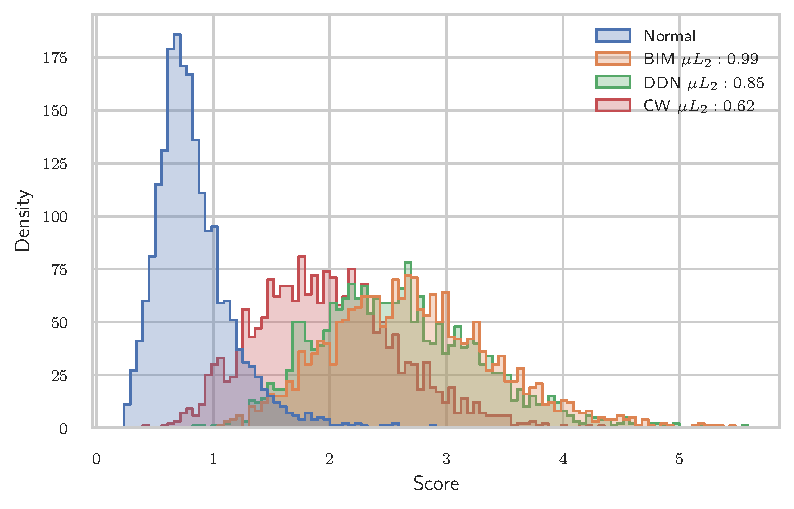
\includegraphics[clip,width=\columnwidth]{Figures/methodology/Fig5a.pdf}%
    }

    \subfloat[Normal images compared with BIM-generated samples at varying
        perturbation budgets.]{%
        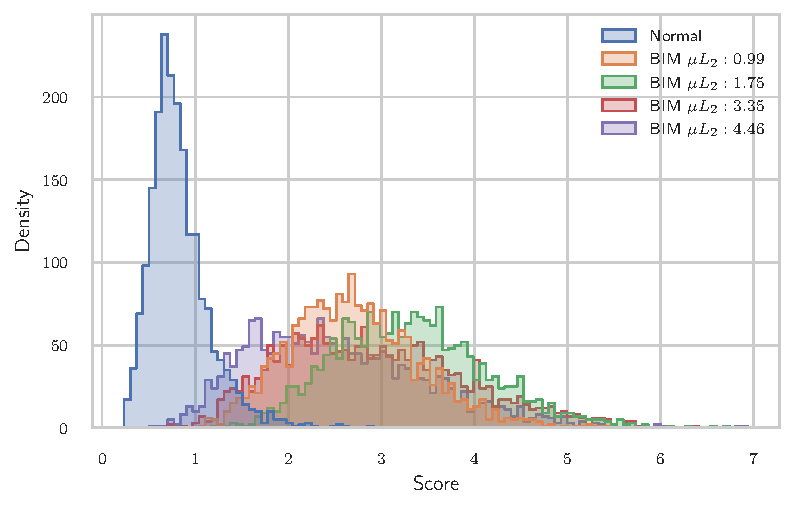
\includegraphics[clip,width=\columnwidth]{Figures/methodology/Fig5b.pdf}%
    }

    \caption{Histograms showing the $score_{1}$ per sample type.}
    \label{fig:score_1}
\end{figure}


\begin{figure}[htp]
    \subfloat[Normal images compared with different adversarial examples
        generation methods.]{%
        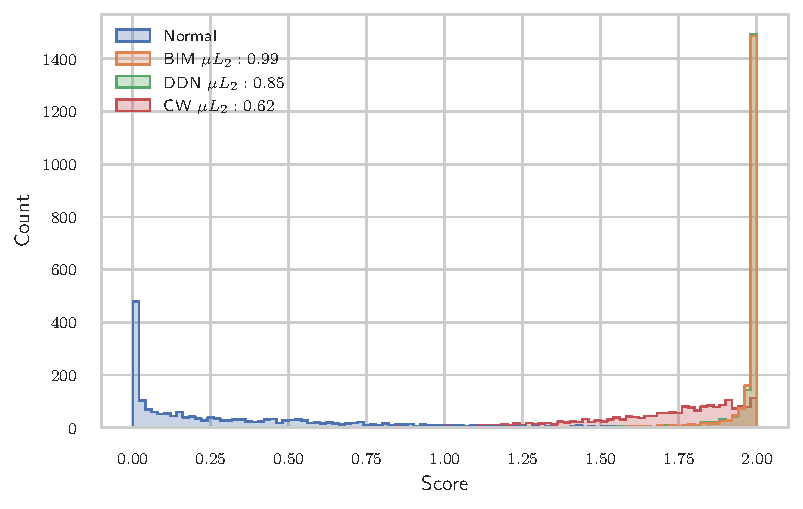
\includegraphics[clip,width=\columnwidth]{Figures/methodology/Fig6a.pdf}%
    }

    \subfloat[Normal images compared with BIM-generated samples at varying
        perturbation budgets.]{%
        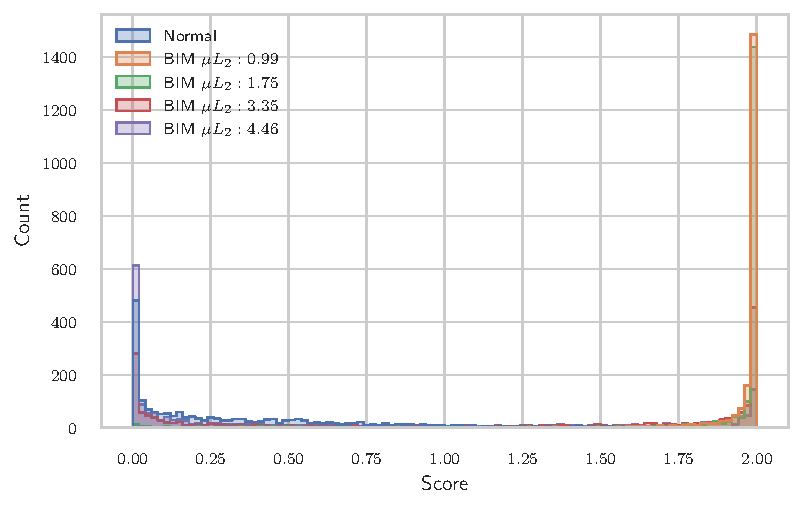
\includegraphics[clip,width=\columnwidth]{Figures/methodology/Fig6b.pdf}%
    }

    \caption{Histograms showing the $score_{2}$ per sample type.}
    \label{fig:score_2}
\end{figure}

As seen in figures \ref{fig:score_1} and \ref{fig:score_2}, using a $\kappa$ of
$0.03$, we observe the distribution of normal images and adversarial examples
differs. However, we can observe in \ref{fig:score_2}B that when the
perturbation budget increases, the distribution of adversarial samples starts to
join the same distribution as normal images. Each score performs differently for
various attacking methods and perturbation budgets. Notably, $score_{1}$ seem to
be less affected by the perturbation budgets of the attacks, offering a better
generalization.

\newpage

\section{Threshold-based Detection: A Method-Specific Approach}
\label{sec:method_specific_approach}
\begin{figure}[htp]
    \subfloat[$score_1$ ImageNet]{%
        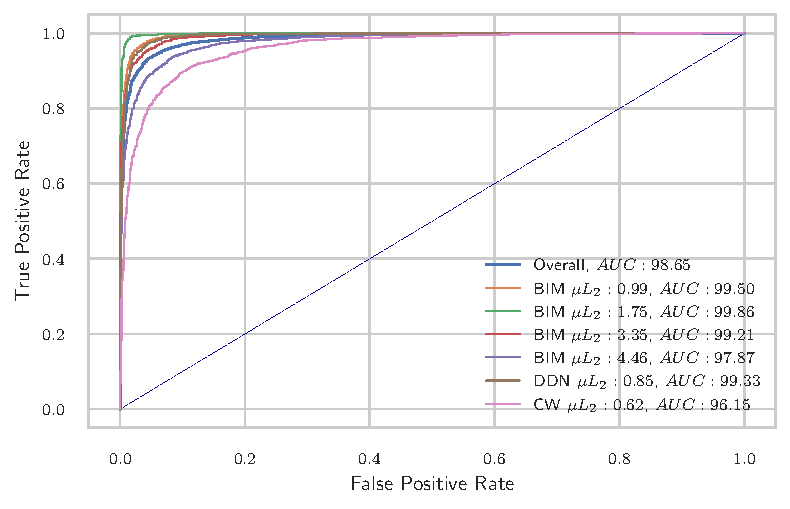
\includegraphics[clip,width=.5\columnwidth]{Figures/methodology/Fig7a.pdf}%
    }
    \subfloat[$score_2$ ImageNet]{%
        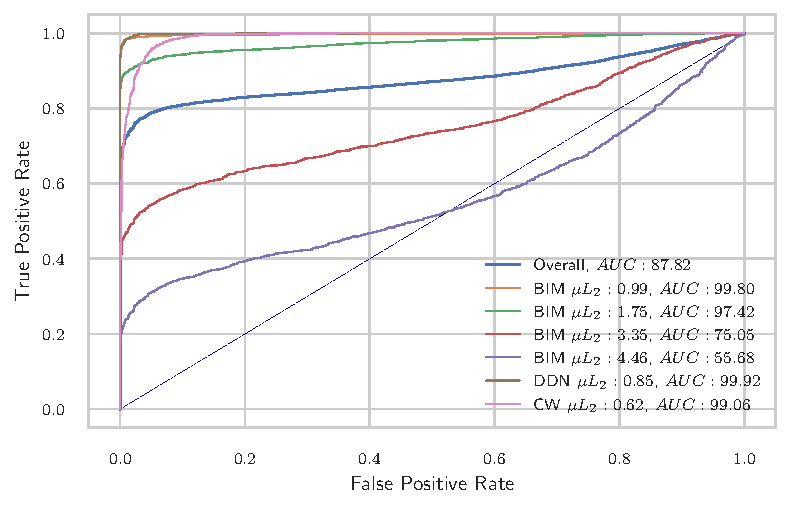
\includegraphics[clip,width=.5\columnwidth]{Figures/methodology/Fig7d.pdf}%
    }

    \subfloat[$score_1$ D. vs. C.]{%
        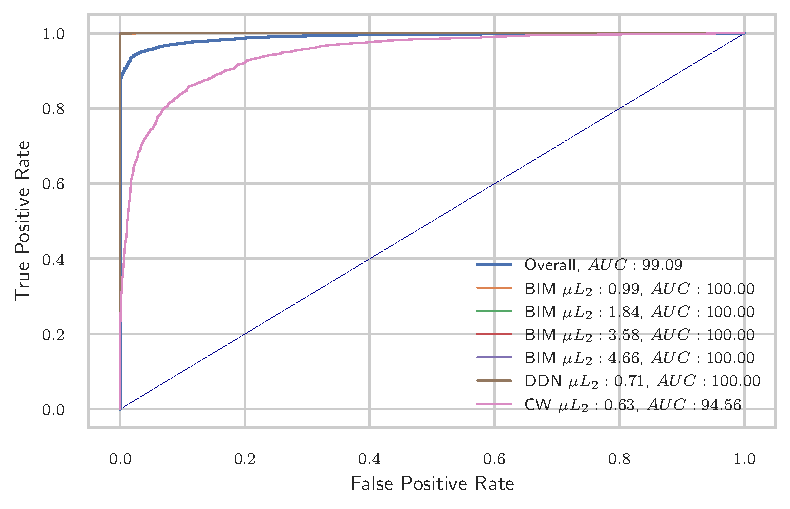
\includegraphics[clip,width=.5\columnwidth]{Figures/methodology/Fig7b.pdf}%
    } \subfloat[$score_2$ D. vs. C.]{%
        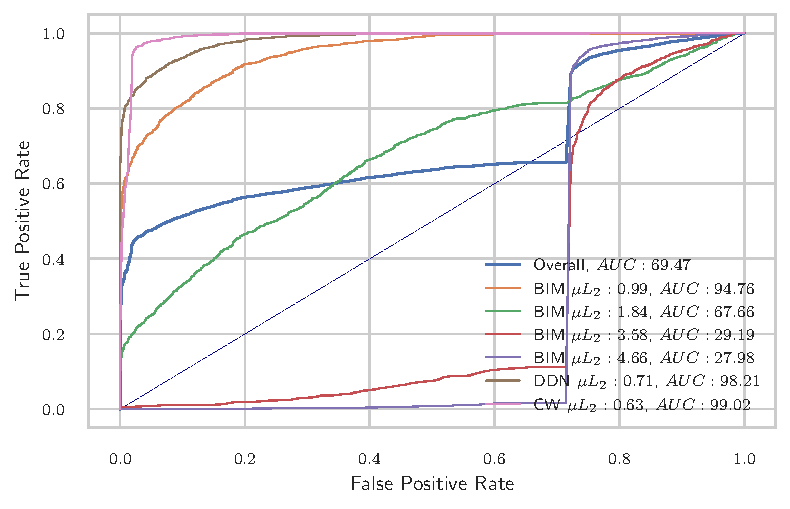
\includegraphics[clip,width=.5\columnwidth]{Figures/methodology/Fig7e.pdf}%
    }

    \subfloat[$score_1$ CIFAR-10]{%
        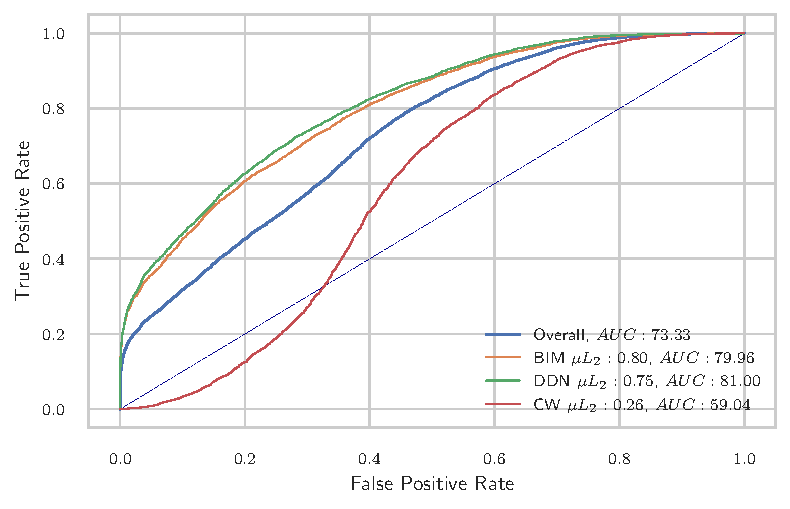
\includegraphics[clip,width=.5\columnwidth]{Figures/methodology/Fig7c.pdf}%
    }
    \subfloat[$score_2$ CIFAR-10]{%
        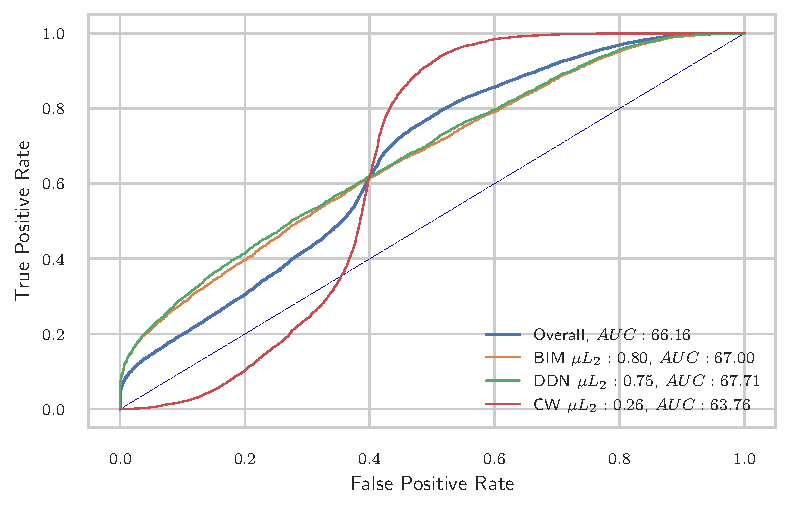
\includegraphics[clip,width=.5\columnwidth]{Figures/methodology/Fig7f.pdf}%
    }
    \caption{ROC-AUC for each classifier and each dataset.}
    \label{fig:rocs}
\end{figure}

To demonstrate the effectiveness of each metric in a detection scenario, we
build a threshold-based binary classifier for each attacking method on each
dataset. The classifiers can either classify an input as negative (normal
images) or positive (adversarial example). Figure \ref{fig:rocs} shows the
Receiver Operating Characteristic Curve (ROC) and Area Under the Curve (AUC) of
each classifier. Following my previous observations, we verify again that
$score_1$ can effectively identify adversarial examples from diverse methods and
even at different perturbation sizes, showing an overall AUC of 98.65\% on
ImageNet and 99.09\% on Dogs vs. Cats.

\section{Adapting to Production: Method-Agnostic Approach}
This method-specific approach described previously is suitable for displaying
each classifier's best available result. Unfortunately, it is not a realistic
scenario in a production environment as we would not be aware of the exact
nature of the input. Furthermore, it would require training a classifier for
each attack method at different perturbation sizes.

I propose an approach to select a threshold for the metric scores, only relying
on the normal images present in the initial datasets to solve this problem. This
approach offers great flexibility and adaptability as we do not require prior
knowledge of the attacking method used to generate an adversarial sample. It is
essential to select a suitable threshold as the detection effectiveness depends
ultimately on it; if the threshold is too high, the number of false positives
will be high and vice versa for false negatives.

\subsection{Threshold and Noise Intensity Selection}
\label{sec:selection_of_the_intensity}

Because of the relation between adversarial and random perturbation discussed in
Section \ref{sub:consistency}, to identify adversarial samples with diverse
adversarial budgets, we also need to generate random perturbations with a wide
range of intensity. To do so, I arbitrarily create a linearly spaced vector
containing ten $\kappa$ from \num{1e-2} to \num{1e-1} and accordingly generate
ten noisy images per given input. For each input pair $x$ and
$\{\tilde{x}\}_{i=1}^{10}$, I compute both $score_1$ (Eq. \ref{eq:score1}) and
$score_2$ (Eq. \ref{eq:score2}). The objective is to detect if a sample has an
abnormally large value with either of the scores.

To determine if a sample has an abnormally large value, we need to select a
threshold for each score \emph{i.e.,} at each noise intensity. To select these
thresholds, I first select 3000 training images from each dataset and record the
scores at each $\kappa$. The thresholds are then placed at the $99_{th}$ percentile
of these scores obtained on training images. Because the thresholds for each
score are determined solely using normal training images, my method does not
require prior knowledge of the attack to perform well.

I use BIM, DDN, and CW attack methods to validate this approach and generate 300
adversarial examples from images present in the ImageNet test set. I also select
100 normal images for the negative samples set.

Figure \ref{fig:distributions_scores} shows how many times each input was
positively detected. As expected, we can observe that most normal images are not
identified as positive once. In contrast, most adversarial examples are
identified as positive at least once. Note that, because we compute $score_1$
and $score_2$ at each ten selected $\kappa$, a sample can be identified from
zero to twenty times as positive.

\begin{figure}[p]
    \centering
    \subfloat[$score_1$]{%
        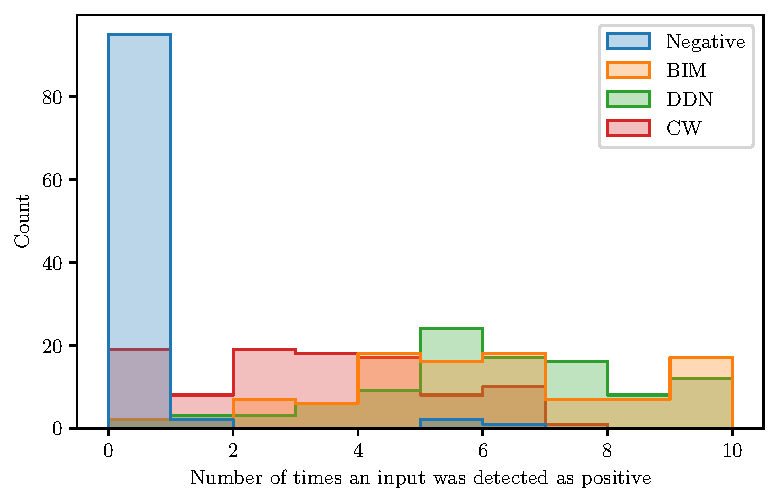
\includegraphics[clip,width=.7\textwidth]{Figures/methodology/distri_1.pdf}
    }

    \subfloat[$score_2$]{%
        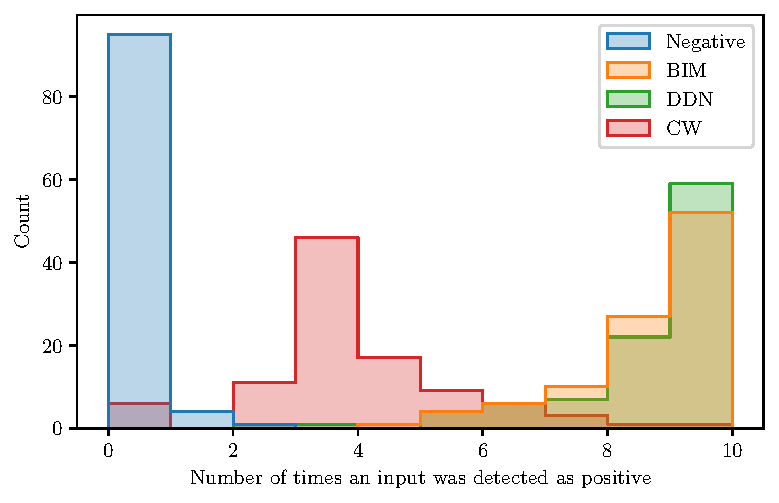
\includegraphics[clip,width=.7\textwidth]{Figures/methodology/distri_2.pdf}
    }

    \subfloat[Scores combined]{%
        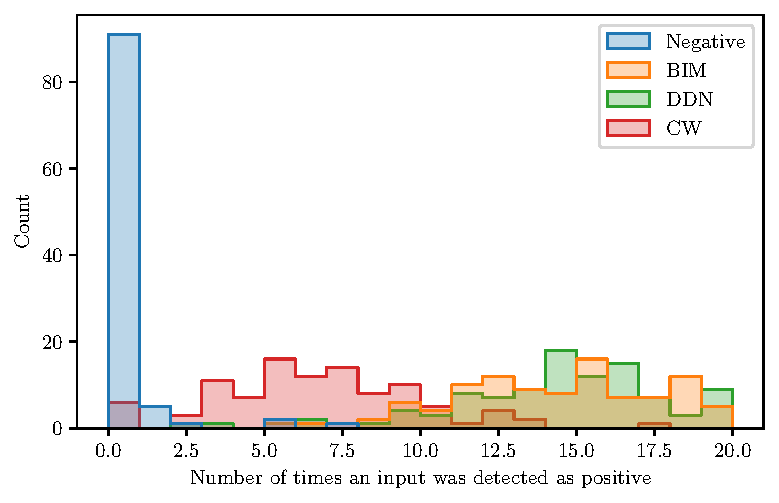
\includegraphics[clip,width=.7\textwidth]{Figures/methodology/distri_combined.pdf}
    } \caption{Histograms showing the number of times an input was detected as
        positive on ImageNet.}
    \label{fig:distributions_scores}
\end{figure}

\newpage

\section{Detection Results and Performance Analysis}
\label{sec:detection_results}

Following the same procedure as in section \ref{sec:selection_of_the_intensity},
I evaluate the method with adversarial examples generated using different
approaches and various perturbation budgets. Table \ref{tab:detection_results}
shows the results of this evaluation. Using the combined scores, I observed a
high overall recall rate of 98.5\% on ImageNet and 100\% on Dogs vs. Cats. The
efficacy of each score depends on the type of attack used; for example,
$score_2$ does not perform as well on untargeted attacks but always performs
better on CW adversarial examples than $score_1$.

We also note that combining the scores shows to be a good strategy: for the cost
of a slight decrease in precision, the recall rate improves as well as the
overall $F_{\beta}$ score. With BIM, increasing the perturbation budget from an
average $L_2$ perturbation of $\approx 1.00$ to $\approx 3.00$ does not affect
the detection precision performances (Table \ref{tab:detection_results},
ImageNet/Dogs vs. Cats, No. 1- 3.).

Commonly, detection precision is higher when facing adversarial examples with
smaller perturbation sizes, such as samples generated with the CW attack method.
For instance, W. Xu \emph{et al} measure the $L_1$ distance between the
prediction vectors of the original image and its squeezed version
\cite{xu_feature_2018}, using bit depth reduction as well as local and non-local
spatial smoothing. As a result, they show comparable detection rates on
adversarial examples generated with the CW method, whereas the detection rate
falls to 55.56\% on samples crafted with BIM. However, using the same attack
settings (BIM$_\infty$, average $L_2$ of $\approx 1.40$), my approach
demonstrates a 100.0\% detection rate using the combined scores (Table
\ref{tab:detection_results}, ImageNet, No. 5). Therefore, a strength of my
method is that it can detect both low-perturbation and large-perturbation
adversarial examples.

This adaptability of our approach comes from the inputs being transformed with
varying random perturbation intensities, which allows for the detection of
samples generated with CW (at lower $\kappa$ values) and the detection of BIM or
similar methods (at higher $\kappa$ values). As seen in Table
\ref{tab:detection_results}, even when increasing the number of iterations from
100 (ImageNet, No. 7) to 10000 (ImageNet, No. 8) for samples generated with the
CW method, the detection performance remains unchanged. This is expected as
increasing the number of iterations does not make the perturbation more robust;
it only makes it less noticeable to the human eye.

\begin{table}[tph]
    \centering
    \begin{adjustbox}{angle=90}
        \resizebox{1.39\linewidth}{!}{%
            \begin{tabular}{c|c|cc|ccc|ccc|ccc|ccc}
                \toprule
                \multicolumn{1}{c}{\multirow{2}{*}{\rotcell{}}}         &
                \multirow{2}{*}{No.}                                    &
                \multirow{2}{*}{Attack}                                 &
                \multirow{2}{*}{$L_{2}$}                                & \multicolumn{3}{c|}{TP}        &
                \multicolumn{3}{c|}{Precision}                          & \multicolumn{3}{c|}{Recall}    &
                \multicolumn{3}{c}{$F_{\beta}$}                                                                           \\
                \multicolumn{1}{c}{}                                    &
                                                                        &                                &      &
                $score_1$
                                                                        &
                $score_2$
                                                                        &
                $combined$
                                                                        &
                $score_1$
                                                                        &
                $score_2$
                                                                        &
                $combined$
                                                                        &
                $score_1$
                                                                        &
                $score_2$
                                                                        &
                $combined$
                                                                        &
                $score_1$
                                                                        &
                $score_2$
                                                                        &
                $combined$
                \\
                \midrule
                \multirow{8}{*}{\begin{turn}{90}ImageNet\end{turn}}     & 1
                                                                        & \multirow{3}{*}{$BIM_{2}^{t}$} & 1.00 & 98
                                                                        &
                \textbf{100}
                                                                        &
                \textbf{100}
                                                                        & 0.951
                                                                        &
                \textbf{0.952}
                                                                        & 0.917
                                                                        & 0.980
                                                                        &
                \textbf{1.000}
                                                                        &
                \textbf{1.000}
                                                                        & 0.974
                                                                        &
                \textbf{0.990}
                                                                        & 0.982
                \\
                                                                        & 2
                                                                        &
                                                                        & 2.00                           &
                99
                                                                        &
                \textbf{100}
                                                                        &
                \textbf{100}
                                                                        &
                \textbf{0.952}
                                                                        &
                \textbf{0.952}
                                                                        & 0.917
                                                                        & 0.990                          &
                \textbf{1.000}
                                                                        &
                \textbf{1.000}
                                                                        & 0.982
                                                                        &
                \textbf{0.990}
                                                                        & 0.982
                \\
                                                                        & 3
                                                                        &
                                                                        & 3.00                           &
                95
                                                                        &
                \textbf{100}
                                                                        &
                \textbf{100}
                                                                        & 0.950
                                                                        &
                \textbf{0.952}
                                                                        & 0.917
                                                                        & 0.950                          &
                \textbf{1.000}
                                                                        &
                \textbf{1.000}
                                                                        & 0.950
                                                                        &
                \textbf{0.990}
                                                                        & 0.982
                \\
                                                                        & 4
                                                                        & $BIM_{2}$                      & 1.00
                                                                        & 96                             & 63
                                                                        &
                \textbf{98}
                                                                        &
                \textbf{0.950}
                                                                        & 0.926
                                                                        & 0.916                          &
                0.960                                                   & 0.630
                                                                        &
                \textbf{0.956}
                                                                        & 0.958
                                                                        & 0.673                          &
                \textbf{0.966}
                \\
                                                                        & 5
                                                                        & $BIM_{\infty}$                 & 1.40 & 99 & 70
                                                                        &
                \textbf{100}
                                                                        &
                \textbf{0.952}
                                                                        & 0.937
                                                                        & 0.917                          &
                0.990                                                   & 0.700
                                                                        &
                \textbf{1.000}
                                                                        &
                \textbf{0.982}
                                                                        & 0.737
                                                                        &
                \textbf{0.982}
                \\
                                                                        & 6
                                                                        & $DDN_{2}^{t}$                  & 0.85 & 98 &
                \textbf{100}
                                                                        &
                \textbf{100}
                                                                        & 0.951
                                                                        &
                \textbf{0.952}
                                                                        & 0.917
                                                                        & 0.980                          &
                \textbf{1.000}
                                                                        &
                \textbf{1.000}
                                                                        & 0.974
                                                                        &
                \textbf{0.990}
                                                                        & 0.982
                \\
                                                                        & 7
                                                                        & $CW_{2}^{t}$                   & 0.46 & 81 &
                \textbf{94}
                                                                        &
                \textbf{94}
                                                                        & 0.942
                                                                        &
                \textbf{0.949}
                                                                        & 0.913
                                                                        & 0.810                          &
                \textbf{0.940}
                                                                        &
                \textbf{0.940}
                                                                        & 0.833
                                                                        &
                \textbf{0.942}
                                                                        & 0.934
                \\
                                                                        & 8
                                                                        & $CW_{2}^{t}*$                  & 0.40 & 88 &
                \textbf{98}
                                                                        &
                \textbf{98}
                                                                        &
                \textbf{0.957}
                                                                        & 0.951
                                                                        & 0.925                          &
                0.880                                                   &
                \textbf{0.980}
                                                                        &
                \textbf{0.980}
                                                                        & 0.894
                                                                        &
                \textbf{0.974}
                                                                        & 0.968
                \\
                \midrule
                \multicolumn{4}{c|}{Total / Average}                    & 754
                                                                        & 725                            &
                \textbf{790}
                                                                        &
                \textbf{0.951}
                                                                        & 0.946
                                                                        & 0.918
                                                                        & 0.943
                                                                        & 0.906
                                                                        &
                \textbf{0.985}
                                                                        & 0.944
                                                                        & 0.911
                                                                        &
                \textbf{0.973}
                \\
                \midrule
                \multirow{5}{*}{\begin{turn}{90}Dogs vs Cats\end{turn}} & 1
                                                                        & \multirow{3}{*}{$BIM_{2}$}     & 1.00 &
                \textbf{100}
                                                                        & 72                             &
                \textbf{100}
                                                                        &
                \textbf{0.962}
                                                                        & 0.935
                                                                        & 0.926
                                                                        &
                \textbf{1.000}
                                                                        & 0.720
                                                                        &
                \textbf{1.000}
                                                                        &
                \textbf{0.992}
                                                                        & 0.755
                                                                        & 0.984
                \\
                                                                        & 2
                                                                        &
                                                                        & 2.00                           &
                \textbf{100}
                                                                        & 46
                                                                        &
                \textbf{100}
                                                                        &
                \textbf{0.962}
                                                                        & 0.902
                                                                        & 0.926                          &
                \textbf{1.000}
                                                                        & 0.460
                                                                        &
                \textbf{1.000}
                                                                        &
                \textbf{0.992}
                                                                        & 0.510
                                                                        & 0.984
                \\
                                                                        & 3
                                                                        &
                                                                        & 3.00                           &
                \textbf{100}
                                                                        & 41
                                                                        &
                \textbf{100}
                                                                        &
                \textbf{0.962}
                                                                        & 0.891
                                                                        & 0.926                          &
                \textbf{1.000}
                                                                        & 0.410
                                                                        &
                \textbf{1.000}
                                                                        &
                \textbf{0.992}
                                                                        & 0.460
                                                                        & 0.984
                \\
                                                                        & 4
                                                                        & $DDN_{2}$                      & 0.71
                                                                        &
                \textbf{100}
                                                                        & 88
                                                                        &
                \textbf{100}
                                                                        &
                \textbf{0.962}
                                                                        & 0.946
                                                                        & 0.926                          &
                \textbf{1.000}
                                                                        & 0.880
                                                                        &
                \textbf{1.000}
                                                                        &
                \textbf{0.992}
                                                                        & 0.892
                                                                        & 0.984
                \\
                                                                        & 5
                                                                        & CW$_{2}$                       & 0.53
                                                                        & 91                             & 99
                                                                        &
                \textbf{100}
                                                                        &
                \textbf{0.958}
                                                                        & 0.952
                                                                        & 0.926                          &
                0.910                                                   & 0.990
                                                                        &
                \textbf{1.000}
                                                                        & 0.919
                                                                        &
                \textbf{0.982}
                                                                        & 0.984
                \\
                \hline
                \multicolumn{4}{c|}{Total / Average}                    & 491
                                                                        & 346                            &
                \textbf{500}
                                                                        &
                \textbf{0.961}
                                                                        & 0.925
                                                                        & 0.926
                                                                        & 0.982
                                                                        & 0.692
                                                                        &
                \textbf{1.000}
                                                                        & 0.977
                                                                        & 0.720
                                                                        &
                \textbf{0.984}
                \\
                \midrule
                \multirow{6}{*}{\begin{turn}{90}CIFAR-10\end{turn}}     & 1
                                                                        & $BIM_{2}^{t}$                  & 0.75 &
                \textbf{67}
                                                                        & 46                             &
                \textbf{67}
                                                                        &
                \textbf{0.882}
                                                                        & 0.754
                                                                        & 0.798
                                                                        & 0.857
                                                                        & 0.460
                                                                        &
                \textbf{0.670}
                                                                        &
                \textbf{0.704}
                                                                        & 0.499
                                                                        & 0.692
                \\
                                                                        & 2
                                                                        & $BIM_{2}$                      & 0.75
                                                                        &
                \textbf{78}
                                                                        & 34
                                                                        &
                \textbf{78}
                                                                        &
                \textbf{0.897}
                                                                        & 0.694
                                                                        & 0.821                          &
                0.857                                                   & 0.340
                                                                        &
                \textbf{0.780}
                                                                        &
                \textbf{0.801}
                                                                        & 0.379
                                                                        & 0.788
                \\
                                                                        & 3
                                                                        & $BIM_{\infty}$                 & 1.00 &
                \textbf{85}
                                                                        & 40
                                                                        &
                \textbf{85}
                                                                        &
                \textbf{0.904}
                                                                        & 0.727
                                                                        & 0.833                          &
                0.857                                                   & 0.400
                                                                        &
                \textbf{0.850}
                                                                        &
                \textbf{0.860}
                                                                        & 0.440
                                                                        & 0.847
                \\
                                                                        & 4
                                                                        & $DDN_{2}$                      & 0.60
                                                                        & 78                             & 47
                                                                        &
                \textbf{79}
                                                                        &
                \textbf{0.897}
                                                                        & 0.758
                                                                        & 0.823                          &
                0.780                                                   & 0.470
                                                                        &
                \textbf{0.790}
                                                                        &
                \textbf{0.801}
                                                                        & 0.509
                                                                        & 0.796
                \\
                                                                        & 5
                                                                        & $CW_{2}$                       & 0.10
                                                                        & 28                             &
                \textbf{89}
                                                                        &
                \textbf{89}
                                                                        & 0.757
                                                                        &
                \textbf{0.856}
                                                                        & 0.840
                                                                        & 0.280                          &
                \textbf{0.890}
                                                                        &
                \textbf{0.890}
                                                                        & 0.320
                                                                        &
                \textbf{0.883}
                                                                        & 0.879
                \\
                                                                        & 6
                                                                        & $CW_{2}^{t}$                   & 0.22 & 37 &
                \textbf{82}
                                                                        &
                \textbf{82}
                                                                        & 0.804
                                                                        &
                \textbf{0.845}
                                                                        & 0.828
                                                                        & 0.370                          &
                \textbf{0.820}
                                                                        &
                \textbf{0.820}
                                                                        & 0.415
                                                                        &
                \textbf{0.825}
                                                                        & 0.822
                \\
                \midrule
                \multicolumn{4}{c|}{Total / Average}                    & 373
                                                                        & 338                            &
                \textbf{480}
                                                                        &
                \textbf{0.857}
                                                                        & 0.772
                                                                        & 0.824
                                                                        & 0.622
                                                                        & 0.563
                                                                        &
                \textbf{0.800}
                                                                        & 0.650
                                                                        & 0.589
                                                                        &
                \textbf{0.804}
                \\
                \bottomrule
            \end{tabular}
        }
    \end{adjustbox}
    \caption{Detection results for each dataset. Results are shown for both
        scores individually ($score_1$ and $score_2$) and combined ($combined$).
        For each attack, we specify the metric with which it was created
        ($\infty$ or $2$), whether the attack is targeted ($t$), and the
        corresponding average $L_2$ distance. \label{tab:detection_results}}
\end{table}

\pagebreak
\subsection{A Real-World Example: Showcasing the Method on a Sample}
To visualize a concrete example, I randomly select one image from the ImageNet
validation set where I perform the previously described method. I then generate
an adversarial example using BIM. Figure \ref{fig:showcase_example_samples}
shows the base image (A), the adversarial perturbation (B) magnified by ten, and
the final result adversarial example (C) that is identified as a "running shoe"
by the model.

\begin{figure}[htp]
    \subfloat[]{%
        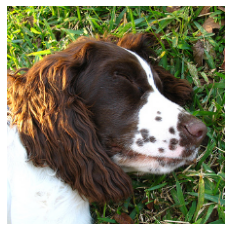
\includegraphics[clip,width=.33\linewidth]{Figures/showcase_example/normal.png}%
    } \subfloat[]{%
        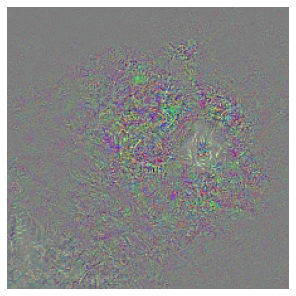
\includegraphics[clip,width=.33\linewidth]{Figures/showcase_example/ae_diff.png}%
    } \subfloat[]{%
        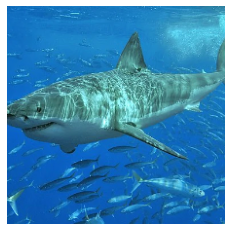
\includegraphics[clip,width=.33\linewidth]{Figures/showcase_example/ae.png}%
    }

    \caption{ Normal image (A), adversarial perturbation (magnified by 10) (B), adversarial example (C). }
    \label{fig:showcase_example_samples}
\end{figure}

\begin{figure}[htp]
    \subfloat[]{%
        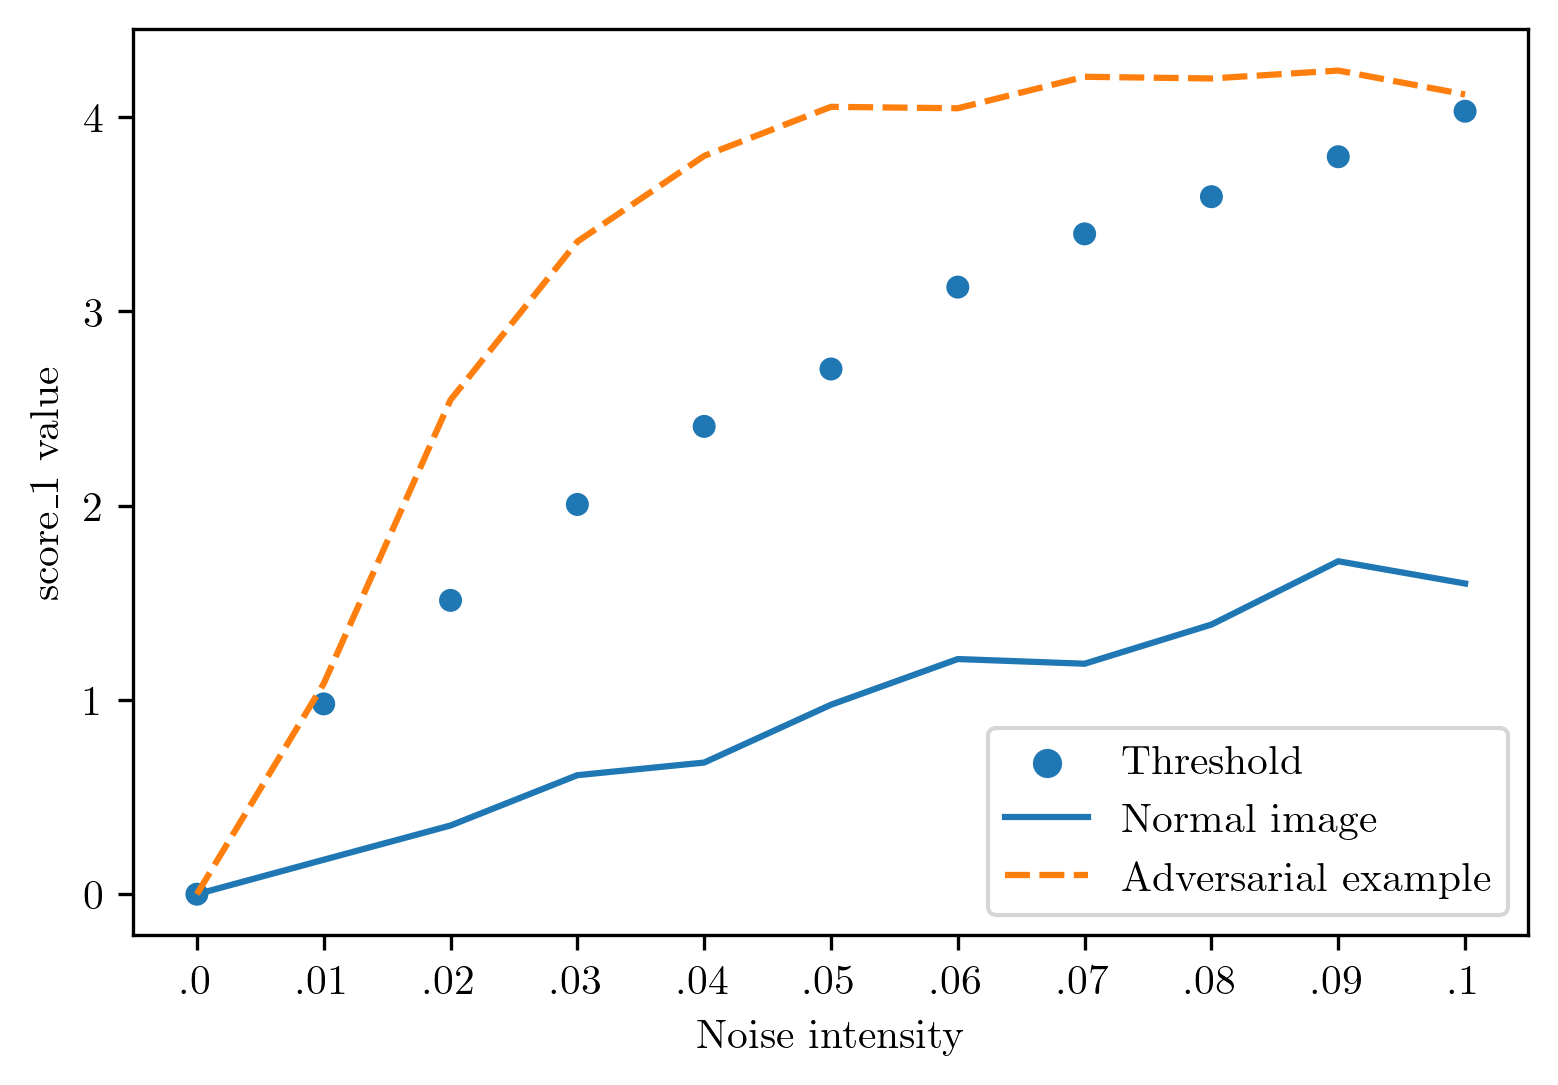
\includegraphics[clip,width=.5\linewidth]{Figures/showcase_example/score_1_threshold.png}%
    } \subfloat[]{%
        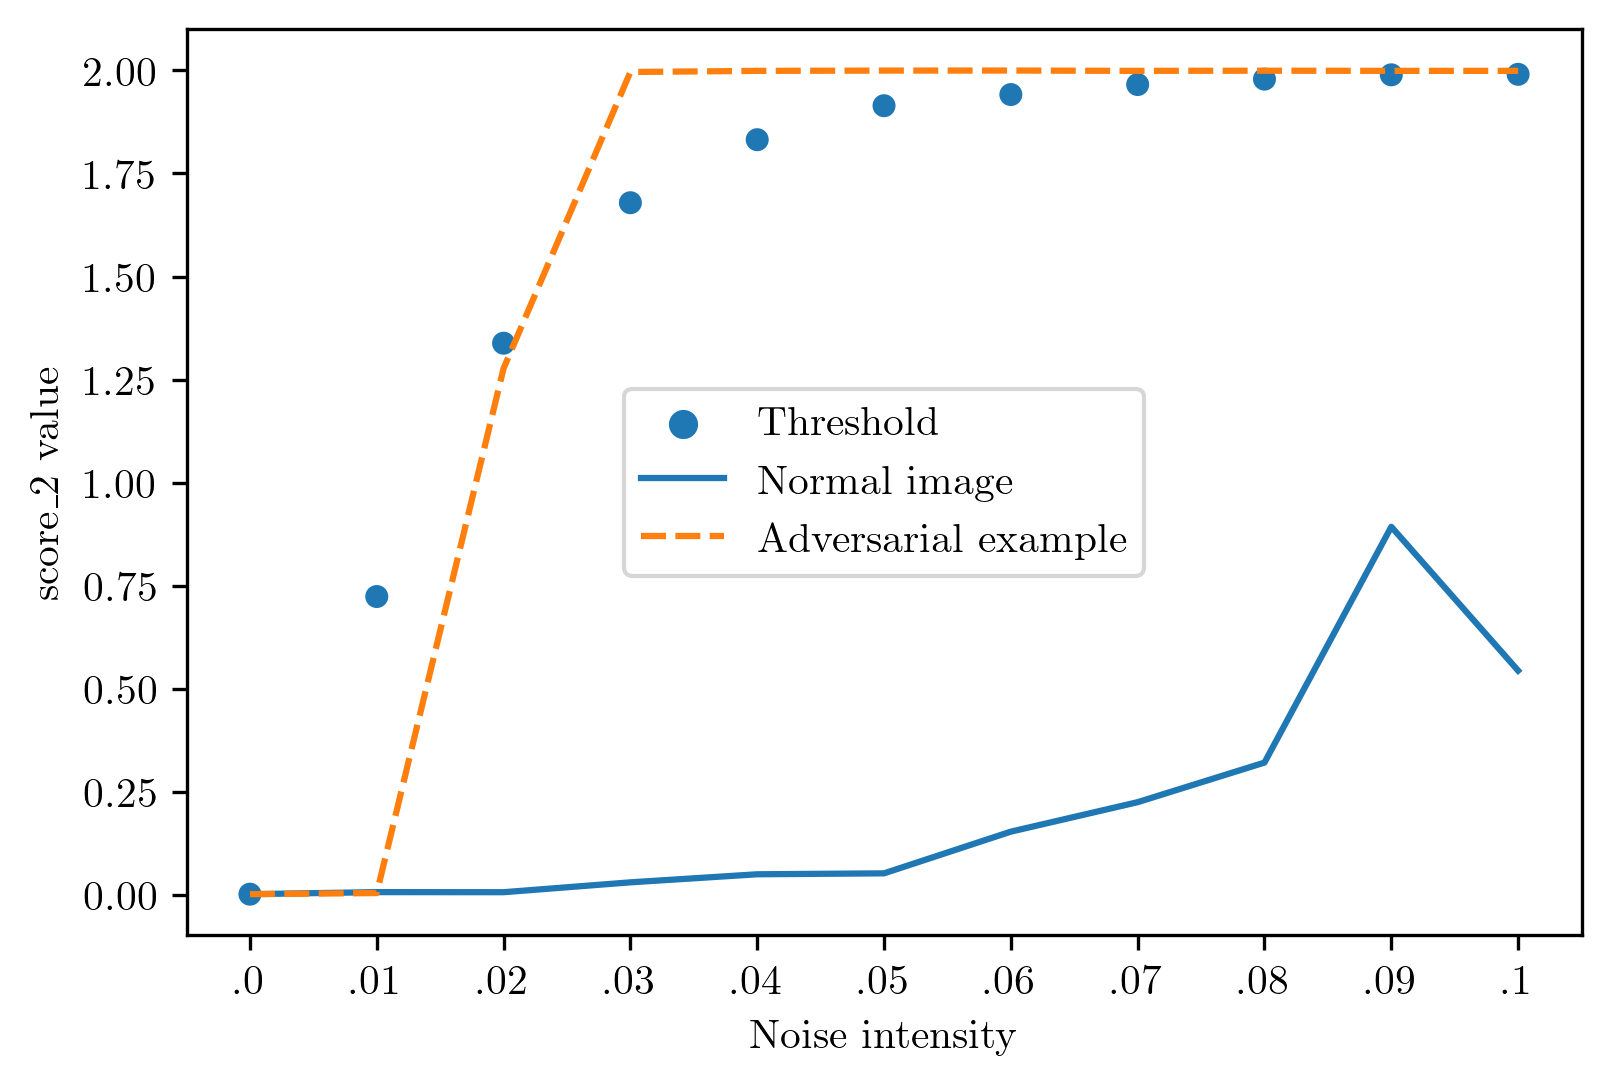
\includegraphics[clip,width=.5\linewidth]{Figures/showcase_example/score_2_threshold.png}%
    }

    \caption{ comparing the number of times the thresholds are respected between
        a normal image and an adversarial example. $score_1$ in (A), $score_2$ in
        (B).  }
    \label{fig:showcase_scores}
\end{figure}

Processing \ref{fig:showcase_example_samples}A and
\ref{fig:showcase_example_samples}B through my approach gives us the results
shown in figure \ref{fig:showcase_scores}. Plot (A) shows us when a sample's
$score_1$ values exceed the threshold values. As expected and verified at the
beginning of this section, the normal image's scores values stay under the
corresponding thresholds. In contrast, the scores of the adversarial examples
exceed the thresholds in a few points; remember that exceeding the threshold at
any given noise intensity is enough to tag the image as being positive,
\emph{i.e.,} adversarial.

Similarly, with figure \ref{fig:showcase_scores}B, where we can
observe the same scenario happening, thresholds are exceeded by the adversarial
example while the normal image's scores remain under them.
